\documentclass[journal]{IEEEtran}
\usepackage{blindtext}
\usepackage{graphicx}
\usepackage{listings}
\usepackage{csquotes}
\usepackage{siunitx}
\usepackage[superscript,biblabel]{cite}


\hyphenation{op-tical net-works semi-conduc-tor}

\begin{document}

\title{Counting Complexity}

\author{Breck~Yunits% <-this % stops a space
\thanks{Breck Yunits is a researcher at Ohayo Computer (breck@ohayo.computer)}% <-this % stops a space
}

\markboth{December~2017 DRAFT}%
{Shell \MakeLowercase{\textit{et al.}}: Bare Demo of IEEEtran.cls for Journals}

\maketitle


\begin{abstract}
%\boldmath
Yet another method for counting complexity.
\end{abstract}

\IEEEpeerreviewmaketitle

\section{Introduction}

\begin{displayquote}
``...make the irreducible basic elements as simple and as few as possible without having to surrender the adequate representation of a single datum of experience.''
- On the Method of Theoretical Physics, Albert Einstein

\end{displayquote}

The above quote is commonly paraphrased as ``Make things as simple as possible, but not simpler.'' This statement presents a hard problem. How do we know when we've made things as simple as possible? How do you count complexity?

One 1999 survey of complexity measures found 48 systems in use \cite{Edmonds}. Despite the abundance of proposed systems, some of which have proved useful in isolated domains, no general measurement system has emerged as a defacto standard \cite{Mitchell}.

In this paper I add to the pile, and propose using Tree Notation as a tool for counting complexity.

\section{An Overview}

The method introduced here, named Tree Notation Complexity (TNC), can be used to measure the complexity of an entity X. It operates as follows.

First, it is assumed that all ideas are graphs that can be sliced into tree structures.

Second, given the assumption that all structures can be represented as trees, we can then use Tree Notation, a simple encoding of tree structures, to encode the components of X, in a program P, which is written in a high level symbolic Tree Notation language defined by a grammar, G0.

Third, we can then describe that language G0 in a recursive series of grammars (G1, G2, ...).

Fourth, we can then stop at a desired level of abstraction (to get Relative Complexity), or continue until we reach irreducible trees (to get Total Complexity).

Fifth, we can use simple arithmetic to count the atomic components of our program and grammars and get complexity measurements for a system.

\section{Simple Examples}

Which concept is more complex, a boolean digit (0 or 1) or a base-10 digit (between 0 and 9)?

Let's imagine a machine that takes as input one character and returns true if that input is defined in a program written for that machine.

Let's encode both concepts using one Tree Notation language (not defined here).

\begin{lstlisting}
boolean
 0
 1
digit
 0
 1
 2
 3
 4
 5
 6
 7
 8
 9
\end{lstlisting}

Comparing the count of nodes, we get two nodes for the "boolean" and ten nodes for the "digit". Hence, by this simple TNC measure we can say that a digit is more complex than a boolean.

Next, let's imagine a similar string matching program that returns true on "pat,pit,pin,bat,bit,bin,fat,fit,fin". In this example, we use two different machines that implement two different languages. The programming language for MachineA can accept only one letter per node. The language for MachineB can accept multiple characters per node and will test its input against each character.


\begin{lstlisting}
programA
 p
  a
   t
  i
   n
 b
  a
   t
  i
   n
 f
  a
   t
  i
   n
programB
 pbf
  ai
   tn
\end{lstlisting}

\begin{figure}[ht!]
\centering
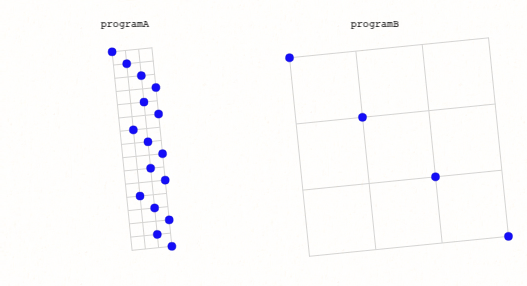
\includegraphics[width=90mm]{programs.png}
\caption{A visualization of the nodes of the two programs above.}
\end{figure}

Both programs are equivalent in that they both will return the same thing for the same input. ProgramA requires fifteen nodes while programB requires three nodes. Hence, the programB is less complex by this measure, given machineA and machineB. I will explain later what I mean by "given machineA and machineB".

\section{Atomic Components of Complexity}

TNC has more atomic units to count beyond nodes. In TNC the five countable atomic units of complexity are trees (files/2D planes), nodes (lines in a file), words (delimited by spaces), edges (line indentation), and word edges (words that are pointers to other nodes). Other derived measures could be devised as well, but in this paper we look at only the atomic units fully necessary to describe an entity.

\begin{figure}[ht!]
\centering
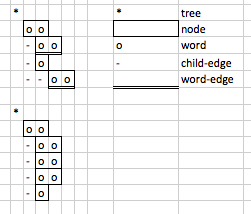
\includegraphics[width=90mm]{atomicUnits.png}
\caption{A visualization of the countable atomic units in TNC.}
\end{figure}


\section{Relative vs Total Complexity}

In the example above, programB was less complex than programA "given machineA and machineB".

However, if we were measuring Total Complexity of programA and programB, we might find that programA is less complex, as the complexity of the tree representation of machineA might be less complex than the complexity of the tree representation of machineB. Total Complexity of an entity aggregates the complexity of the tree representation of the entity along with the tree representations of all its dependencies.

Another trivial example might be, given a computer that can execute both C code and Python code, and a task to sum some numbers from a CSV file, a program in Python would be less complex. But the Total Complexity of the Python program might be greater than that of the C program, when dependencies are measured.


\section{Why Tree Notation?}

TNC is one of many systems that measure the "difficulty of description" \cite{Lloyd}--the entity isn't measured directly, rather the description of the entity is measured.

Tree Notation is used because it can easily describe micro and macro concepts, and a user can zoom between macro and micro scales as easily as moving within scales.

Basic primitives like the bit, the concept of a word, or an AND gate have a Tree Notation representation.

Macro objects, like the Linux Kernel, could also be described using just Tree Notation.

Both the description and the grammars the description uses are represented by the same basic minimal structures allowing the whole system to be counted and analyzed.

Tree Notation is minimal and unambiguous. Descriptions written in Tree Notation can expand gracefully to handle new ideas. Other descriptions become noisier or repetitive over time, whereas Tree Notation is a noiseless encoding and the signal in the information remains strong over time.

Tree Notation is a universal notation that can describe items in any domain, from computer science and mathematics to medicine and the law. TNC thus could enable cross-domain complexity comparisons.

In a sense, Tree Notation can be thought of as a notation for building a strongly-typed noiseless encyclopedia, and then the complexity of items in that encylopedia can then be measured and compared.

Furthermore, items encoded in Tree Notation can be thought of and visualized as existing in 3-Dimensions. This is far-off speculation, but perhaps there exists a correlation between the TNC measurements of a topic, and the number of neurons and synapses dedicated to that topic in the brain of a topic expert, out of the total supply of their \num{10e11} neurons and \num{10e15} synapses.

\section{Big Complexity}

How complex is the U.S. tax code? How complex is the Linux Kernel? How complex is a comprehensive description of the human brain? How complex is a comprehensive blueprint of the new iPhone?

At the moment no total complexity descriptive project so ambitious has been attempted in Tree Notation. It is an open question as to whether or not such an accomplishment is even possible. For example, a back of the envelope estimate of how many nodes might be in the total Tree Notation description of the Linux Kernel might be a \num{10e6} or perhaps as many as \num{10e12}.

One thing is certain: assuming Tree Notation does provide the simplest notation to describe entities and thus measure their complexity (a big assumption), that does not change the fact that the total complexity of entities in our modern world is large and ever increasing.

\section{Growth of Complexity}

The Total Complexity of the world increases monotonically over time in terms of raw atomic units like tree, node and edge counts. However, new higher level trees are also constantly introduced, reducing Relative complexity in many areas at the same time that absolute complexity generally increases. Relative Complexity measurements of concepts ebbs and flows in sinusoidal waves, while the underlying absolute complexity steadily increases.

\section{Conclusion and Future Work}

To an evergrowing number of systems for measuring I add one more: Tree Notation Complexity. The benefit of this system is that it is simple, practical, universal, and scale free. Future projects might look at creating Tree Notation descriptions of large, complex systems and visualizing and summarizing the results.

\begin{thebibliography}{4}

\bibitem{Edmonds}
Edmonds, B. (1999). Syntactic Measures of Complexity. Doctoral Thesis, University of Manchester, Manchester, UK.

\bibitem{Mitchell}
Mitchell, M., 2009. Complexity: A guided tour. Oxford University Press.

\bibitem{Lloyd}
Lloyd, Seth. "Measures of complexity: a nonexhaustive list." IEEE Control Systems Magazine 21.4 (2001): 7-8.

\end{thebibliography}


\end{document}
